\documentclass[mat1, tisk]{fmfdelo}
\usepackage{graphicx}
\usepackage{enumitem}
% \documentclass[fin1, tisk]{fmfdelo}
% Če pobrišete možnost tisk, bodo povezave obarvane,
% na začetku pa ne bo praznih strani po naslovu, …

%%%%%%%%%%%%%%%%%%%%%%%%%%%%%%%%%%%%%%%%%%%%%%%%%%%%%%%%%%%%%%%%%%%%%%%%%%%%%%%
% METAPODATKI
%%%%%%%%%%%%%%%%%%%%%%%%%%%%%%%%%%%%%%%%%%%%%%%%%%%%%%%%%%%%%%%%%%%%%%%%%%%%%%%

% - vaše ime
\avtor{Tadeja Možina}

% - naslov dela v slovenščini
\naslov{Metrična dimenzija grafa deliteljev niča}

% - naslov dela v angleščini
\title{Metric dimension of a zero-divisor graph}

% - ime mentorja/mentorice s polnim nazivom:
%   - doc.~dr.~Ime Priimek
%   - izr.~prof.~dr.~Ime Priimek
%   - prof.~dr.~Ime Priimek
%   za druge variante uporabite ustrezne ukaze
\mentor{izr.~prof.~dr.~David Dolžan}

% - leto diplome
\letnica{2024} 

% - povzetek v slovenščini
%   V povzetku na kratko opišite vsebinske rezultate dela. Sem ne sodi razlaga
%   organizacije dela, torej v katerem razdelku je kaj, pač pa le opis vsebine.
\povzetek{V diplomski nalogi preučujemo metrično dimenzijo grafa deliteljev niča.}

% - povzetek v angleščini
\abstract{In this thesis, we study the metric dimension of a zero-divisor graph.}

% - klasifikacijske oznake, ločene z vejicami
%   Oznake, ki opisujejo področje dela, so dostopne na strani https://www.ams.org/msc/
\klasifikacija{74B05, 65N99}

% - ključne besede, ki nastopajo v delu, ločene s \sep
\kljucnebesede{naravni logaritem\sep nenaravni algoritem}

% - angleški prevod ključnih besed
\keywords{natural logarithm\sep unnatural algorithm} % angleški prevod ključnih besed

% - angleško-slovenski slovar strokovnih izrazov
\slovar{
\geslo{continuous}{zvezen}
\geslo{uniformly continuous}{enakomerno zvezen}
\geslo{compact}{kompakten -- metrični prostor je kompakten, če ima v njem vsako zaporedje stekališče; podmnožica evklidskega prostora je kompaktna natanko tedaj, ko je omejena in zaprta  }
\geslo{glide reflection}{zrcalni zdrs ali zrcalni pomik -- tip ravninske evklidske izometrije, ki je kompozitum zrcaljenja in translacije vzdolž iste premice}  
\geslo{lattice}{mreža}  
\geslo{link}{splet}
\geslo{partition}{\textbf{$\sim$ of a set} razdelitev množice; \textbf{$\sim$ of a number} razčlenitev števila}
}

% - ime datoteke z viri (vključno s končnico .bib), če uporabljate BibTeX
\literatura{literatura.bib}

%%%%%%%%%%%%%%%%%%%%%%%%%%%%%%%%%%%%%%%%%%%%%%%%%%%%%%%%%%%%%%%%%%%%%%%%%%%%%%%
% DODATNE DEFINICIJE
%%%%%%%%%%%%%%%%%%%%%%%%%%%%%%%%%%%%%%%%%%%%%%%%%%%%%%%%%%%%%%%%%%%%%%%%%%%%%%%

% naložite dodatne pakete, ki jih potrebujete
\usepackage{algpseudocode}  % za psevdokodo
\usepackage{algorithm}      % za algoritme
\floatname{algorithm}{Algoritem}
\renewcommand{\listalgorithmname}{Kazalo algoritmov}

% deklarirajte vse matematične operatorje, da jih bo LaTeX pravilno stavil
% \DeclareMathOperator{\conv}{conv}
% na razpolago so naslednja matematična okolja, ki jih kličemo s parom
% \begin{imeokolja}[morebitni komentar v oklepaju] ... \end{imeokolja}
%
% definicija, opomba, primer, zgled, lema, trditev, izrek, posledica, dokaz

% za številske množice uporabite naslednje simbole
\newcommand{\R}{\mathbb R}
\newcommand{\N}{\mathbb N}
\newcommand{\Z}{\mathbb Z}
% Lahko se zgodi, da je ukaz \C definiral že paket hyperref,
% zato dobite napako: Command \C already defined.
% V tem primeru namesto ukaza \newcommand uporabite \renewcommand
\newcommand{\C}{\mathbb C}
\newcommand{\Q}{\mathbb Q}

%%%%%%%%%%%%%%%%%%%%%%%%%%%%%%%%%%%%%%%%%%%%%%%%%%%%%%%%%%%%%%%%%%%%%%%%%%%%%%%
% ZAČETEK VSEBINE
%%%%%%%%%%%%%%%%%%%%%%%%%%%%%%%%%%%%%%%%%%%%%%%%%%%%%%%%%%%%%%%%%%%%%%%%%%%%%%%

\begin{document}

\section{Uvod}

%Na začetku prvega poglavja/razdelka (ali v samostojnem razdelku z naslovom
%Uvod) napišite kratek zgodovinski in matematični uvod. Pojasnite motivacijo za
%problem, kje nastopa, kje vse je bil obravnavan. Na koncu opišite tudi
%organizacijo dela -- kaj je v kakšnem razdelku.

%Če se uvod naravno nadaljuje v besedilo prvega poglavja, lahko nadaljujete z
%besedilom v istem razdelku, sicer začnete novega. Na začetku vsakega
%razdelka/podraz\-delka poveste, čemu se bomo posvetili v nadaljevanju. Pri
%pisanju uporabljajte ukaze za matematična okolja, med formalnimi enotami
%dodajte vezno razlagalno besedilo.
Pojem metrične dimenzije grafa je v sedemdesetih letih prejšnjega stoletja 
uvedel Peter J. Slater, problem iskanja le te pa sta kot prva raziskovala 
Frank Harary in Robert Melter~\cite{7dolzan}~\cite{4pirzada17}. Uporablja se 
na različnih področjih, kot na primer v farmacevtski kemiji, navigaciji 
robotov in kombinatorični optimizaciji~\cite{0OuSh}.
%
%
\section{1}
V tem poglavju bomo predstavili osnovne pojme, povezane z metrično dimenzijo grafa 
deliteljev niča. Pri tem bomo sledili~\cite{0OuSh}. Skozi celotno diplomsko nalogo 
bodo bili vsi grafi neusmerjeni.
%
\subsection{Osnovne definicije}
%
\begin{definicija}
  Naj bo R kolobar in $Z(R)$ njegova množica deliteljev niča.
  \emph{Graf deliteljev niča kolobarja R} je enostaven neusmerjen graf z množico
  vozlišč $Z^{*}(R) = Z(R)\setminus\{0\} $, kjer sta dve različni vozlišči $a,b \in R $
  povezani natanko tedaj, ko je $ab = 0$ ali $ba = 0$. Označimo ga z $\Gamma(R)$.
\end{definicija}
%
\begin{zgled}\label{prim1}
  Poglejmo si graf deliteljev niča kolobarja $\Z_{10}$. Množica njegovih vozlišč je 
  $V(\Gamma(\Z_{10})) = Z^{*}(\Z_{10}) = \{2, 4, 5, 6, 8\}$, množica povezav pa 
  je enaka $E(\Gamma(\Z_{10})) = \{2 - 5, 4 - 5, 5 - 6, 5 - 8\}$.
  \begin{figure}[H]
    \centering
    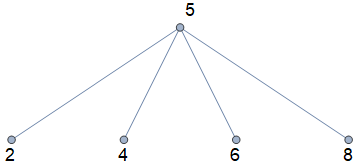
\includegraphics[scale=0.5]{z10.png}
    \caption{Graf deliteljev niča $\Z_{10}$}
  \end{figure}
\end{zgled}
%
\begin{zgled}\label{zgled2.3}
  Poglejmo si še graf deliteljev niča kolobarja $\Z_{12}$. Množica njegovih vozlišč je 
  $V(\Gamma(\Z_{12})) = Z^{*}(\Z_{12}) = \{2, 3, 4, 6, 8, 9, 10\}$, povezave pa so 
  prikazane na sliki.
  \begin{figure}[H]
    \centering
    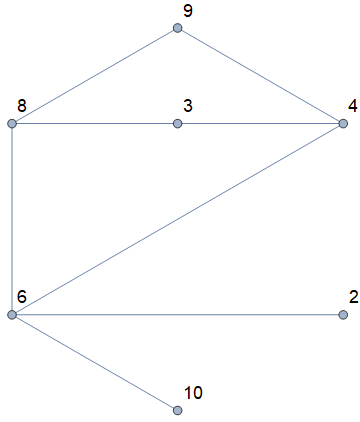
\includegraphics[scale=0.5]{z12.png}
    \caption{Graf deliteljev niča $\Z_{12}$}
  \end{figure}
\end{zgled}
%
Spomnimo se še definicije razdalje med dvema vozliščema v grafu. Za poljubni vozlišči 
$u,v \in V(\Gamma)$ je \emph{razdalja} med $u$ in $v$, označena z $d(u,v)$, dolžina 
najkrajše poti med njima. Če ne obstaja pot med $u$ in $v$, je $d(u,v) = \infty $.
Z uporabo te definiramo predstavitev $v$ glede na $W$.
%
\begin{definicija}
  Naj bo $W = \{ w_1,w_2, \ldots, w_k \}$ urejena podmnožica od $V(\Gamma)$ in 
  $v \in V(\Gamma)$. Potem 
  se $k$-dimenzionalni vektor $r(v|W)=( d(v,w_1), \ldots, d(v,w_k) )$ imenuje 
  \emph{predstavitev $v$ glede na $W$}. 

  Rečemo, da je $v$ \emph{rešljiv z W}, če velja $r(v|W) \neq r(u|W)$, 
  za vsak $u \in V(\Gamma)$ različen od $v$, torej 
  $( d(v,w_1), \ldots, d(v,w_k) ) \neq ( d(u,w_1), \ldots, d(u,w_k) )$ za vsak 
  $u \neq v$.
\end{definicija}
%
Množici $W$ pravimo \emph{rešljiva množica od $\Gamma$}, če imata poljubni različni 
vozlišči v $V(\Gamma)$ različni predstavitvi glede na $W$. Če je $W$ rešljiva množica 
z najmanjšo močjo, ji pravimo \emph{baza od $\Gamma$}.
%
%Metrična dimenzija
\begin{definicija}
  \emph{Metrična dimenzija grafa $\Gamma$} je moč njene baze. Označimo jo z $dim(\Gamma)$.
\end{definicija}
%
\begin{opomba}\label{opomba2.7}
  %dovolj je gledati predstavitve elementov izven W glede na W.
  Če preverjamo, ali je $W= \{w_1,w_2, \ldots, w_k\}$ podmnožica od $V(\Gamma)$ 
  rešljiva množica $\Gamma$, je dovolj gledati predstavitve elementov iz 
  $V(\Gamma) \setminus W$ glede na $W$. Namreč če vzamemo $w_i \in W$ bo 
  $(d(w_i,w_1),d(w_i,w_2), \ldots d(w_i,w_k))$ na $i$-tem mestu imela 0. 
  Če bi katerokoli drugo vozlišče $u$ imelo enako predstavitev kot $w_i$, bi 
  potem moralo veljati, da $d(w_i,w_i) = d(u,w_i)$, kar pa je edino možno, 
  če je $u = w_i$.
\end{opomba}
%
\begin{opomba}\label{opomba2.8}
  Očitno je vsaka nadmnožica rešljive množice grafa $\Gamma$ tudi sama rešljiva 
  množica. Res, naj bo $W_2$ nadmnožica rešljive množice $W_1$ grafa $\Gamma$, 
  torej $W_1 \subseteq W_2$. Po opombi \ref{opomba2.7} je dovolj gledati 
  predstavitve elementov izven $W_2$. Ker so predstavitve teh elementov glede na 
  $W_1$ različne in $W_2$ vsebuje $W_1$, bodo njihove predstavitve glede na 
  $W_2$ bile enake tistim v $W_1$ z nekaj dodanimi komponentami, torej še vedno 
  različne.
\end{opomba}
%
\begin{zgled}\label{prim1.2}
  Poiščimo metrično dimenzijo grafa deliteljev niča kolobarja $\Z_{10}$ iz 
  primera \ref{prim1}. Razdalje 
  med dvema poljubnima različnima vozliščema so 1 ali 2. Če za $W = \{w\}$ vzamemo 
  katerokoli enoelementno množico, bosta obstajali vsaj dve vozlišči iz 
  $\{2,4,6,8\}$, ki imata enako razdaljo do $w$, torej to ni baza. Podoben razmislek 
  naredimo, če je $W$ dvoelementna množica - v $\{2,4,6,8\}$ bosta obstajali dve 
  vozlišči z enako predstavitvijo glede na $W$. Poglejmo sedaj, če obstaja rešljiva 
  množica moči 3. Vzemimo $W = \{2,4,6\}$. Edina dva elementa, ki ju rabimo pogledati 
  sta 5 in 8. Izračunamo 
  $(d(5,2),d(5,4),d(5,6)) = (1,1,1) \neq (d(8,2),d(8,4),d(8,6)) = (2,2,2)$. Torej je 
  metrična dimenzija $\Gamma(\Z_{10})$ = 3.
\end{zgled}
%
\begin{opomba}
  Graf $\Gamma$ ima lahko več rešljivih množic iste moči. Pri zgledu \ref{prim1.2} 
  bi za rešljivo množico moči 3 (in torej tudi bazo) tako lahko vzeli tudi 
  $\{2,4,8\}$, $\{2,6,8\}$ ali $\{4,6,8\}$.
\end{opomba}
%
\subsection{Meje metrične dimenzije grafa}
%
Ponovimo nekaj pojmov, ki jih bomo potrebovali v nadaljevanju. Za graf 
$\Gamma = (V, E)$ je njegov \emph{premer}, označen z $diam(\Gamma)$, največja 
razdalja med dvema vozliščema v grafu. \emph{Soseščina} vozlišča $v$ je 
množica $N(v) = \{ x \in V(\Gamma)~|~x \sim v \}$, torej množica vozlišč 
s katerimi ima $v$ povezavo. 

Navedimo sedaj prvo trditev, ki postavi meje metrične dimenzije grafa~\cite{10chartrand}.
%
\begin{trditev}
  Naj bo $\Gamma$ povezan graf z $n$ vozlišči in premerom $d$ = $diam(\Gamma)$. Potem velja
  $n - d^{dim(\Gamma)} \leq dim(\Gamma) \leq n - d$.
\end{trditev}
\begin{dokaz}
  Poglejmo si najprej drugo neenakost. Naj bosta $u$ in $v$ vozlišči grafa 
  $\Gamma$, pri katerih je razdalja največja možna, torej $d(u,v) = d$. 
  Njuno $uv$-pot dolžine $d$ zapišemo kot $u=v_0, v_1, \ldots, v_d=v$. 
  Naj bo $W = V(\Gamma) \setminus \{v_1, \ldots, v_d \}$. Potem je 
  $d(u,v_i) = i$ za $i = 1, \ldots, d$. Ker je $u \in W$ in imajo 
  vsa vozlišča grafa izven $W$ paroma različno razdaljo do $u$ in 
  torej različno predstavitev glede na $W$, je $W$ 
  rešljiva množica od $\Gamma$.

  Za dokaz prve neenakosti izberimo bazo $B$ od $\Gamma$ moči $k$. 
  Poglejmo vozlišča iz $V(\Gamma) \setminus B$, teh je $n-k$. 
  Njihove predstavitve 
  glede na $B$ so vektorji dolžine $k$, katerih koordinate so števila med 
  $1$ in $d$. Vsakemu vozlišču iz $V(\Gamma) \setminus B$ priredimo 
  tak vektor. Ker je $B$ baza, morajo biti vektorji med sabo različni. 
  Torej je preslikava injektivna in dobimo $n - k \leq d^k$. 
  Neenakost preuredimo in dobimo željen rezultat.
\end{dokaz}
%
Navedimo še nekaj novih definicij, s katerimi si bomo pomagali še dodatno 
izboljšati meje metrične dimenzije grafa.
%
\begin{definicija}
  Za vozlišči $u, v\in V(\Gamma)$ pravimo, da sta \emph{dvojčka}, če velja 
  $N(u) \cup \{u\} = N(v) \cup \{v\} $, ko $u \sim v$, ali 
  $N(u) = N(v) $, ko $u \nsim v$.

  Množici vseh dvojčkov vozlišča $v$ rečemo \emph{množica dvojčkov vozlišča $v$}. 
  Označimo jo z $Tw(v)$.
\end{definicija}
%
Opazimo, da $V(\Gamma)$ lahko zapišemo kot disjunktno unijo množic 
dvojčkov, saj vsaka množica dvojčkov $Tw(v)$ vsebuje vsaj en element, vozlišče $v$.
Glede na to, koliko vozlišč vsebujejo, množice dvojčkov delimo v dve skupini.
%
\begin{definicija}
  Množici dvojčkov $Tw(v)$ pravimo, da je \emph{prava množica dvojčkov grafa $\Gamma$}, 
  če je $|Tw(v)| \geq 2$. Če je $|Tw(v)| = 1$, ji rečemo 
  \emph{osamljena množica dvojčkov grafa $\Gamma$}. 

  Število pravih množic grafa $\Gamma$ označimo z \emph{$\alpha(\Gamma)$}, število 
  osamljenih množic dvojčkov pa z \emph{$\beta(\Gamma)$}.
\end{definicija}
%
\begin{zgled}
  Poglejmo množice dvojčkov iz zgleda \ref{zgled2.3}. Množice dvojčkov so 
  $\{9,3\},$ $\{8,4\},\{2,10\}$ in $\{6\}$. Število pravih množic grafa $\Gamma(\Z_{12})$ 
  je torej $\alpha(\Gamma(\Z_{12})) = 3$, število osamelih pa $\beta(\Gamma(\Z_{12})) = 1$.
\end{zgled}
%
Navedimo sedaj trditev, ki uporabi množice dvojčkov za omejitev metrične 
dimenzije grafa~\cite{3pirzada14}.
%
\begin{trditev}
  Naj bo $\Gamma$ povezan graf in $T_1, T_2, \ldots, T_{\alpha(\Gamma)}$ različne 
  prave množice dvojčkov grafa $\Gamma$. Potem velja:
  \begin{enumerate}[label=(\roman*)]
    \item Vsaka baza od $\Gamma$ vsebuje vsa, razen morda enega, vozlišča iz 
          vsakega $T_i$, za $1 \leq i \leq \alpha(\Gamma)$,
    \item Obstaja baza $P$ od $\Gamma$, da $P$ vsebuje največ $|T_i| - 1$ vozlišč 
          iz vsakega $T_i$, za $1 \leq i \leq \alpha(\Gamma)$,
    \item $|V(\Gamma)| - \alpha(\Gamma) - \beta(\Gamma) \leq dim(\Gamma) \leq |V(\Gamma)| - \alpha(\Gamma)$.
  \end{enumerate}
\end{trditev}
\begin{dokaz}
  Dokažimo najprej točko i). Naj bo $W$ rešljiva množica od $\Gamma$. Recimo, da trditev ne velja, 
  torej da obstajata vozlišči $u,v$ v isti pravi množici dvojčkov, ki nista obadva v $W$. 
  Naj bo ta množica dvojčkov $T_i$. Ker sta $u$ in $v$ v isti množici dvojčkov, 
  imata enake sosede, torej je njuna predstavitev glede na $W$ enaka, kar pa ni 
  možno, saj je $W$ baza.

  Dokažimo sedaj točko ii). Naj bo $B$ rešljiva množica od $\Gamma$ in 
  $T_1, \ldots, T_{\alpha(\Gamma)}$ njene prave množice dvojčkov ter 
  $T_{\alpha(\Gamma)+1}, \ldots, T_{\alpha(\Gamma)+\beta(\Gamma)}$ osamljene množice dvojčkov.
  Poglejmo množico $T_1$. 
  Po točki i) $B$ vsebuje vsa, razen morda enega, vozlišča iz $T_1$. Izberimo $W$ 
  rešljivo množico tako, da bo v celoti vsebovala $T_1$ - če $B$ že v celoti vsebuje 
  $T_1$, je $W = B$, če ne, pa za $W$ izberemo $B$, ki mu dodamo manjkajoče vozlišče in po 
  opombi \ref{opomba2.8} bo ta še vedno rešljiva množica. Naj bo $x \in T_1$ in 
  $W = \{x, w_1, w_2, \ldots\}$. Označimo $P_1 = W \setminus \{x\} = \{w_1, w_2, \ldots\}$ 
  in dokažimo, da je rešljiva množica.
  Vzemimo različni vozlišči $v_1, v_2 \in V(\Gamma)$. Če je vsaj eden izmed njiju v $P_1$, 
  že vemo, da sta njuni predstavitvi glede na $P_1$ različni. Naj bosta sedaj 
  $v_1, v_2 \notin P_1$. Recimo, da je njuna predstavitev 
  glede na $P_1$ enaka, torej $r(v_1|P_1) = r(v_2|P_1)$. Ker je $W$ rešljiva množica, 
  je njuna predstavitev glede na $W$ različna, $r(v_1|W) \neq r(v_2|W)$. Iz 
  tega sledi, da se $r(v_1|P_1)$ in $r(v_2|P_1)$ razlikujeta na prvi komponenti, 
  torej da je $d(x,v_1) \neq d(x,v_2)$. $T_1$ je prava množica dvojčkov, 
  torej obstaja $z \in T_1 $, da $z \neq x$. Ker je $z$ tudi v $P_1$ in 
  $r(v_1|P_1) = r(v_2|P_1)$, sledi, da $d(z,v_1) = d(z,v_2)$. Vendar pa sta 
  $x$ in $z$ v isti pravi množici dvojčkov, torej velja, da 
  $d(x,v_1) = d(z,v_1) = d(z,v_2) = d(x,v_1)$, iz česar pridemo v protislovje. 
  Torej je $P_1$ rešljiva množica grafa $\Gamma$. Postopek ponovimo še za 
  ostale prave množice dvojčkov $T_i$, za $2 \leq i \leq \alpha(\Gamma)$: 
  na $i$-tem koraku množici $P_i$ dopolnimo za največ eno vozlišče tako, da bo 
  v celoti vsebovala $T_i$, nato pa eno (ne nujno isto) vozlišče odstranimo. 
  Ker so prave množice dvojčkov $T_1, \ldots, T_{\alpha(\Gamma)}$ med seboj disjunktne, 
  je ta postopek smiseln.
  Na koncu bo bila $P_{\alpha(\Gamma)}$ rešljiva množica.

  Nazadnje dokažimo še točko iii). Po točki ii) obstaja baza $P$, ki ima iz vsake 
  množice dvojčkov $T_i$, $1 \leq i \leq \alpha(\Gamma)$ največ $|T_i| - 1$ vozlišč. 
  Torej $P$ je baza, ki ima največ $|V(\Gamma)| - \alpha(\Gamma)$ vozlišč in 
  posledično je $dim(\Gamma) \leq |V(\Gamma)| - \alpha(\Gamma)$. Spodnjo mejo dokažimo s 
  pomočjo točke i). Naj bodo $T_1, \ldots, T_{\alpha(\Gamma)}$ prave množice dvojčkov ter 
  $T_{\alpha(\Gamma)+1}, \ldots, T_{\alpha(\Gamma)+\beta(\Gamma)}$ osamljene množice dvojčkov. 
  Po točki i) vsaka baza vsebuje vse, razen morda enega, vozlišča iz 
  $T_1, \ldots, T_{\alpha(\Gamma)}$. Če upoštevamo, da je osamljenih množic $\beta(\Gamma)$, 
  dobimo $|V(\Gamma)| - \alpha(\Gamma) - \beta(\Gamma) \leq dim(\Gamma)$.
\end{dokaz}
%
Poglejmo definicijo določitvenega števila.
%
\begin{definicija}
  Naj bo $\Gamma$ graf z množico vozlišč $V(\Gamma)$. Podmnožica D od $V(\Gamma)$ 
  se imenuje \emph{določitvena množica od $\Gamma$}, če je edini avtomorfizem na 
  $\Gamma$, ki fiksira vsak element v D, identiteta.\\
  Velikosti najmanjše take podmnožice D od $V(\Gamma)$ pravimo 
  \emph{določitveno število $\Gamma$} in ga označimo s $fix(\Gamma)$.
\end{definicija}
%
Označimo še množico 
$O_v = \{ \phi(v) \in V(\Gamma)~|~ \phi \in Aut(\Gamma) \}$ kot 
\emph{orbito} vozlišča $v$ in $O_v = \{ \phi(v) \in V(\Gamma)~|~ \phi \in Aut(\Gamma) \}$
Navedimo trditev, ki velja za določitveno število grafa~\cite{1erwin}.
%
\begin{trditev}
  Naj bo $\Gamma$ graf z netrivialno grupo avtomorfizmov. Potem velja, da 
  je $fix(\Gamma)=1$ natanko tedaj, ko obstaja vozlišče $v \in V(\Gamma)$, 
  da je $|O_v| = |Aut(\Gamma)|$.
\end{trditev}










%\begin{equation}\label{eq:razlika}
%  |x-y|<\delta\quad \text{in}\quad |f(x)-f(y)| \ge \varepsilon. \qedhere
%\end{equation}
%
%V zgornjem primeru smo kvadratek za konec dokaza postavili v zadnjo vrstico
%besedila, ki je vrstična formula, s pomočjo ukaza \verb|\qedhere|.  Ta ukaz
%ustrezno deluje znotraj okolij \emph{equation, align*} in podobnih, ne pa
%znotraj \verb|$$ ... $$|.
%
%Oglejmo si še enkrat neenačbi~\eqref{eq:razlika}. Na formule se sklicujemo z
%ukazom \verb|\eqref{oznaka}|, ki postavi zaporedno številko enačbe
%v oklepaje, na trditve in ostale enote pa z ukazom \verb|\ref{oznaka}|. Črni
%
%Oglejmo si še enkrat neenačbi~\eqref{eq:razlika}. Za sklicevanje na označene
%enote besedila imamo na razpolago dva ukaza; na formule se sklicujemo z ukazom
%\verb|\eqref{oznaka}|, \dots
%
%Če dokaz trditve ne sledi neposredno formulaciji trditve, moramo povedati, kaj
%bomo dokazovali. To naredimo tako, da ob ukazu za okolje dokaz dodamo neobvezni
%parameter,  v katerem napišemo besedilo, ki se bo izpisalo namesto besede
%\emph{Dokaz}, npr.\ \verb|\begin{Dokaz}[Dokaz izreka \ref{izr:enakomerno}]|.
%
%\begin{dokaz}[Dokaz izreka \ref{izr:enakomerno}]
%  Dokazovanja te trditve se lahko lotimo tudi takole \ldots
%\end{dokaz}
%
%\subsection{Naslov morebitnega (pod)razdelka} Besedilo naj se nadaljuje v vrstici naslova, torej za ukazom \verb|\subsection{}| ne smete izpustiti prazne vrstice.
%
%Podobno kot lahko spremenimo ime dokaza, lahko dodamo komentar v ime trditve,
%torej s pomočjo neobveznega parametra; prvega od spodnjih izpisov dosežemo z
%ukazom \verb|\begin{posledica}[izrek o vmesni vrednosti]|. Če želimo v
%parametru navesti vir, pri katerem bomo navedli podatek o tem, kje v viru to
%trditev najdemo, pa uporabimo ukaz
%\verb|\begin{posledica}[\protect{\cite[izrek 3.14]{glob}}]|. Seveda lahko obe
%možnosti kombiniramo.
%
%\begin{posledica}[izrek o vmesni vrednosti]
%  Naj bo $f$ zvezna in \ldots
%\end{posledica}
%
%Ali pa
%
%\begin{posledica}%[izrek o vmesni vrednosti \protect{\cite[izrek 3.14]{glob}}]
%  Naj bo $f$ zvezna in \ldots
%\end{posledica}
%
%Podobno lahko napovemo tudi vsebino primera.
%
%\begin{primer}[nezvezna funkcija nima nujno lastnosti povprečne vrednosti]
%  Naj bo $f \colon \R \to \R$ dana s predpisom \dots
%\end{primer}
%
%\section{Konec dela}
%
%Na konec dela sodita angleško-slovenski slovarček strokovnih izrazov in seznam
%uporabljene literature, morebitne priloge (programska koda, daljša ponovitev
%dela snovi, ki je bil obravnavan med študijem \dots) pa neposredno pred ti
%enoti. Slovar naj vsebuje vse pojme, ki ste jih spoznali ob pripravi dela, pa
%tudi že znane pojme, ki ste jih spoznali pri izbirnih predmetih. Najprej
%navedite angleški pojem (ti naj bodo urejeni po abecedi) in potem ustrezni
%slovenski prevod; zaželeno je, da temu sledi tudi opis pojma, lahko komentar
%ali pojasnilo. Slovarska gesla navajajte z ukazom \verb|\geslo{}{}|, npr.\
%\verb|\geslo{continuous}{zvezen}|.
%
%Pri navajanju literature si pomagajte s spodnjimi primeri; najprej je opisano
%pravilo za vsak tip vira, nato so podani primeri. Člen literature napišete z
%ukazom \verb|\bibitem{oznaka} podatki o viru|, kjer mora \emph{ozmaka} enolično
%določati vir.  Posebej opozarjam, da spletni viri uporabljajo paket url, ki je
%vključen v~.cls datoteki. Polje ``ogled'' pri spletnih virih je obvezno; če je
%kak podatek neznan, ustrezno ``polje'' seveda izpustimo. Literaturo je potrebno
%urediti po abecednem vrstnem redu; najprej navedemo vse vire z znanimi avtorji
%(tiskane in spletne) po abecednem redu avtorjev (po priimkih, nato imenih),
%nato pa spletne vire brez avtorjev, urejene po naslovih strani. Če isti vir
%navajamo v dveh oblikah, kot tiskani in spletni vir, najprej navedemo tiskani
%vir, nato pa še podatek o tem, kje je dostopen v elektronski obliki.
%
\end{document}
